%%%%%%%%%%%%%%%%%%%%%%% file template.tex %%%%%%%%%%%%%%%%%%%%%%%%%
%
% This is a general template file for the LaTeX package SVJour3
% for Springer journals.          Springer Heidelberg 2010/09/16
%
% Copy it to a new file with a new name and use it as the basis
% for your article. Delete % signs as needed.
%
% This template includes a few options for different layouts and
% content for various journals. Please consult a previous issue of
% your journal as needed.
%
%%%%%%%%%%%%%%%%%%%%%%%%%%%%%%%%%%%%%%%%%%%%%%%%%%%%%%%%%%%%%%%%%%%
%
% First comes an example EPS file -- just ignore it and
% proceed on the \documentclass line
% your LaTeX will extract the file if required
\begin{filecontents*}{example.eps}
    %!PS-Adobe-3.0 EPSF-3.0
    %%BoundingBox: 19 19 221 221
    %%CreationDate: Mon Sep 29 1997
    %%Creator: programmed by hand (JK)
    %%EndComments
    gsave
    newpath
    20 20 moveto
    20 220 lineto
    220 220 lineto
    220 20 lineto
    closepath
    2 setlinewidth
    gsave
    .4 setgray fill
    grestore
    stroke
    grestore
\end{filecontents*}
\hyphenation{OpenAI}
\hyphenation{Alpha-Zero}
\hyphenation{Alpha-Star}
%
\RequirePackage{fix-cm}
%
\documentclass{svjour3}                     % onecolumn (standard format)
%\documentclass[smallcondensed]{svjour3}     % onecolumn (ditto)
%\documentclass[smallextended]{svjour3}       % onecolumn (second format)
%\documentclass[twocolumn]{svjour3}          % twocolumn
%
\smartqed  % flush right qed marks, e.g. at end of proof
%
\usepackage{graphicx}
\usepackage{amssymb}
\usepackage{amsmath}
\usepackage[final]{pdfpages}
\usepackage[english]{babel}

%
% \usepackage{mathptmx}      % use Times fonts if available on your TeX system
%
% insert here the call for the packages your document requires
%\usepackage{latexsym}
% etc.
%
% please place your own definitions here and don't use \def but
% \newcommand{}{}
%
% Insert the name of "your journal" with
% \journalname{myjournal}
%

%\newcommand{\argmax}[1]{\underset{#1}{\operatorname{arg}\,\operatorname{max}}\;}
\DeclareMathOperator*{\argmax}{arg\,max} 

\begin{document}

    \title{Model-free Deep Reinforcement Learning -- Algorithms and Applications}
    \subtitle{Reinforcement Learning Seminar -- Winter Semester 2018/19}

    \author{Fabian Otto}

    \institute{Fabian Otto \at
    Technische Universit\"at Darmstadt, Computer Science Department\\
    \email{fabian.otto@stud.tu-darmstadt.de}
    }

    \date{Received: date / Accepted: date}

    \maketitle
    \begin{abstract}
		This survey presents an overview of the current model-free deep reinforcement learning landscape. 
		It provides a comparison of state-of-the-art on-policy and off-policy algorithms in the value-based and policy-based domain.
		Influences and possible drawbacks of different algorithmic approaches are analyzed and associated with new improvements in order to overcome previous problems.
%		This shows a trend towards off-policy learning combined with maximum entropy-based reinforcement learning.
		Further, the survey shows application scenarios for difficult domains, including the game of Go, Starcraft II, Dota 2 and Rubik's Cube.
		\keywords{Deep Reinforcement Learning \and Model-free \and Neural Networks}
    \end{abstract}

    \section{Introduction \label{sec:intro}}
    Artificial neural networks have been used in machine learning since the beginning. 
    The first steps towards today's neural networks can be dated back to McCulloch and Pitts \cite{McCulloch1943}, who published the first work about the operating principles of neurons and created electrical circuits based on this idea.
%     e.\,g. the Dartmouth Summer Research Project on Artificial Intelligence \cite{McCarthy2006}.
	The following advancements of computers and Rosenblatt's invention of the perceptron \cite{Rosenblatt1958} provided a boost to neural networks.  
    Minsky and Papert followed up on this and stated in their book ``Perceptrons'' \cite{Minsky2017} that the perceptron algorithm is not able to learn non-linear behavior such as XOR problems.
%    This led to researchers mostly abandoning neural networks until MADALINE \cite{Winter1988} was able to solve a real world problem.
	The consequent ``AI Winter'' was ended with the introduction of backpropagation \cite{Rumelhart1986}, which provides an easy training procedure for multiple layers, therefore allows to model non-linear functions.
%	It showed an effective way to train neural networks with multiple layers, which allows non-linear functions to be learned.
    Due to the lack of computational resources, the excitement decayed shortly after.
%     the hardware advancements of computers provide sufficient computational power for neural networks.
    More recently this bottleneck could be eliminated and neural networks have shown great success in e.\,g. computer vision \cite{Krizhevsky2012,He2016}, but have also found applications in reinforcement learning, such as the game of Go \cite{Silver2017}, Dota 2 \cite{OpenAI2018} or StarCraft II \cite{Vinyals2019}.
    Based on this success, this survey provides an overview of the current model-free reinforcement learning algorithm landscape for the on-policy and off-policy domain, additionally some notable application examples are presented.
    
    \section{Background\label{sec:background}}
%    \paragraph{Markov Decision Process}
    A \textit{Markov Decision Process} (MDP) is defined as a tuple $(\mathcal{S}, \mathcal{A}, \mathcal{T},\mathcal{R})$, where $\mathcal{S}$ is a finite set of states, $\mathcal{A}$ is a finite set of actions and $\mathcal{T}:\mathcal{S} \times \mathcal{A} \rightarrow \Pi(\mathcal{S})$ represents the state transition function, which returns a probability distribution over states.
    $\mathcal{R}:\mathcal{S} \times \mathcal{A} \rightarrow \mathbb{R}$ provides the expected immediate reward for taking each action in each state. 
    This survey mainly considers the infinite horizon MDP, which tries to maximize the expected discounted cumulative reward:
    \[
    G_t = \mathbb{E} \left[ \sum_{\tau=t}^{\infty} \gamma^{\tau-t} \mathcal{R}(s_\tau,a_\tau)\middle|s_\tau,a_\tau \right]
	\]
    Here $\gamma \in \left[0,1\right)$ describes the discount factor, which trades off immediate and future rewards.
    Reinforcement learning algorithms now aim to find a policy $\pi:\mathcal{S} \rightarrow \mathcal{A}$ which describes the optimal behavior maximizing the expected future reward from all states.
    Consequently, an action-value function which returns the value of taking an action $a$ in state $s$, under the policy $\pi$ is defined as:
    \[
    Q_\pi(s,a) = \mathbb{E}\left[G_t|s_t =s,a_t=a,\pi\right] = \mathcal{R}(s,a) + \gamma \sum_{s\in\mathcal{S}}\mathcal{T}(s,a,s') \max_{a'}Q_\pi(s',a')
	\]
    In order to find the best policy, value-based methods are interested in finding the optimal action-value function $Q^*(s,a) =\max_\pi Q_\pi(s,a)$, which can be computed iteratively by the Bellman operator:
    \[
	 Q_{t+1}(s,a) = \mathcal{R}(s,a) + \gamma \sum_{s\in\mathcal{S}}\mathcal{T}(s,a,s') \max_{a'}Q_t(s',a')
    \]
    When $Q_t \approx Q^*$, the optimal policy can be computed by $\pi^*(s) \approx \argmax_{a} Q_t(s,a)$.
    Alternatively, the optimal value function $V^*(s) = \mathbb{E}\left[G_t|s_t=s, \pi\right] = \max_{a} Q^*(s,a)$ can be used.\\
    In contrast to value-based methods, policy-based methods directly parameterize a policy $\pi(s;\theta)$. 
    One such method is REINFORCE \cite{Williams1992}, it updates the policy parameters $\theta$ in the direction $\nabla_\theta \mathbb{E}[G_t]\approx \nabla_\theta\log\pi(s_t;\theta)G_t$.
    In order to reduce variance and keep the estimate unbiased, a baseline $b(s_t)$ is subtracted from the return $\nabla_\theta\log\pi(s;\theta)(G_t - b(s_t))$. 
    For this baseline, it is common to use an estimate of the value function $b(s_t)\approx V_\pi(s_t)$.
    By applying the policy gradient theorem, $G_t-b(s_t)$ can be seen as an estimate of the advantage function $A_\pi(s_t,a_t) = Q_\pi(s_t,a_t) - V_\pi(s_t)$.
    Combining parameterized policies and value function estimator results in \textit{Actor-Critic} (AC) methods. 
    
    \section{Algorithms \label{sec:algorithms}}
	This section provides an overview of the current deep reinforcement learning landscape including improvements and state-of-the-art algorithms (Figure \ref{fig:overview}). 
	This survey classifies algorithms either as on-policy or off-policy.
	On-policy algorithms estimate the value of the policy while using it for control.
	In contrast, off-policy algorithms utilize a generating policy, called \textit{behavior policy}, and a \textit{target policy}.
	The behavior policy is not necessarily related to the target policy, which is improved and evaluated.
	This allows to use a deterministic target policy, while sampling actions through a stochastic behavior policy. \cite{Sutton2018}
	\begin{figure}[!t]
		\centering
		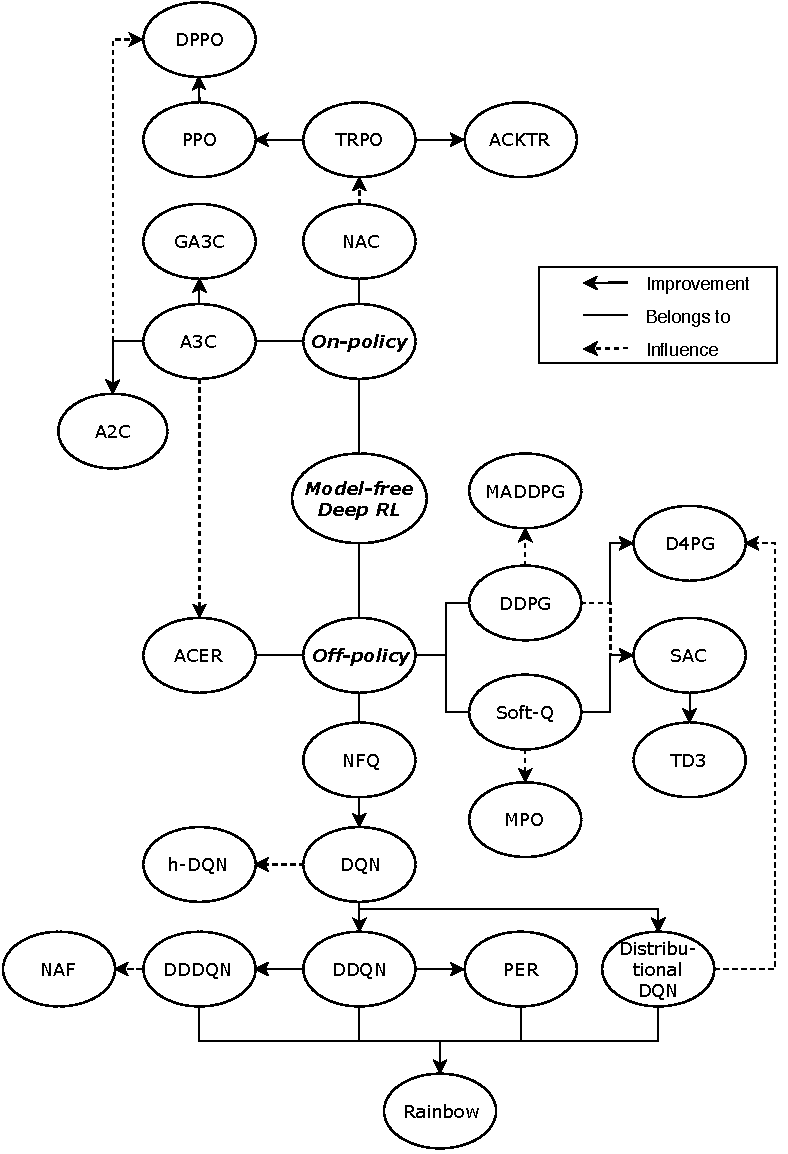
\includegraphics[height=.75\textheight]{images/tree3.pdf}
		\label{fig:overview}
		\caption{Overview of model-free reinforcement learning algorithms.}
	\end{figure}
		
 	\subsection{Off-Policy \label{sec:off-policy}}
	Many current off-policy algorithms are based on the original \textit{Neural Fitted Q-Iteration} (NFQ) \cite{Riedmiller2005} published in 2005. 
	NFQ is based on vanilla Q-Learning \cite{Watkins1989} and approximates the action-value function with a multilayer-perceptron.
	Compared to other approaches at the time, NFQ allows to learn with relatively good sample efficiency.
	Further, batches from a replay memory \cite{Lin1992} are used in order to train the multilayer-perceptron with \textit{Resilient Backpropagation} (RPROP) \cite{Riedmiller1993}.
	Thereby, it is possible to dynamically add new samples to the replay memory during learning.
	Motivated by this idea as well as the success of TD-gammon \cite{Tesauro1994} one of the biggest improvements in deep reinforcement learning, \textit{Deep Q-Networks} (DQN) \cite{Mnih2015}, was introduced.   
	DQN shows human-level performance in multiple games of the Atari Arcade Environment \cite{Bellemare2013}. 
%	They built upon their prior results \cite{Mnih2013} on the Atari Arcade Environment \cite{Bellemare2013} which already achieved state-of-the-art performance for some of the games.
	Compared to NFQ, DQN introduces better scalability to large data sets by replacing RPROP with \textit{Stochastic Gradient Descent} (SGD) updates. 
	Further, DQN allows training end-to-end from the raw visual input utilizing \textit{Convolutional Neural Networks} (CNN). 
%	Benchmarks of the more recent DQN version \cite{Mnih2015} show an improved performance as well as a better generalization to more Atari games compared to the initial work \cite{Mnih2013}.
	However, the key improvement is the introduction of a second target Q-network, which is only periodically updated and thereby reduces sample correlations.\\
	Despite the success, van Hasselt, et al. \cite{VanHasselt2016} show that DQN is not sufficient to avoid overestimation of action-values under certain conditions. 
	This in itself is not harmful to the policy's performance, but if the overestimation is not uniform and not concentrated at the states of interest, it might affect the policy negatively. 
	To mitigate the risk of overestimation, they propose \textit{Double DQN} (DDQN).
	Double Q-Learning \cite{VanHasselt2010} in general decouples the selection and evaluation of actions by learning two action-value functions. 
	One determines the greedy policy and the other the value of this policy.  
	In order to reduce the computational cost, DDQN utilizes the already existing online Q-network for determining the greedy policy and the target Q-network for estimating its value. 
	This allows to achieve better performance on most of the Atari games. 
	Decoupling is also done in a more extreme form with \textit{Dueling Double DQNs} (DDDQN) \cite{Wang2016}. 
	DDDQN represents the action-value by two separate function approximations, a state-value and a state-dependent action-advantage function estimate.
	This representation allows the dueling architecture to learn about the value of a state regardless of the action taken. 
	This is especially important when the action has no repercussions on the near future. 
	Combining DDQN with gradient clipping and \textit{Prioritized Experience Replay} (PER) \cite{Schaul2015} shows that sampling rare experiences with a higher probability makes learning with replay memories even more efficient. 
	However, sampling non-uniformly from the replay memory introduces a bias, that has to be corrected during the update step.
	The \textit{51-atom distributional DQN agent} (C51) \cite{Bellemare2017} does not compute the expected future reward, i.\,e. action-value function, but the corresponding distribution instead. 
	This distributional view allows to reduce chattering and provides a more stable training as well as a rich set of auxiliary predictions.
	Combining different DQN versions in one algorithm shows even better performance and is introduced by \textit{Rainbow} \cite{Hessel2018}.
	The authors additionally present an analysis of the incorporated components and show that all but one result in significantly improved performance.\\
%	A general comparison of different DQN version is presented by Hessel, et al. \cite{Hessel2018}, they also introduce \textit{Rainbow}, combining different DQN improvements in one algorithm.\\
	All previous approaches are using environments, which do not have to deal with delayed and sparse feedback.
	In real world applications this is often not the case and algorithms still need the ability to learn.
	One key problem during training is insufficient exploration, causing unstable policies. 
	Using intrinsically motivated agents, exploration can be achieved through the agent itself rather than through an external objective. 
	This idea is implemented by \textit{hierarchical-DQN} (h-DQN) \cite{Kulkarni2016}.
	A top level meta-controller is selecting a subgoal in order to optimize the extrinsic reward.
	The lower level controller maximizes an intrinsic reward by solving the subgoal.
	This enables h-DQN to achieve a significantly better performance on the Atari game ``Montezuma's Revenge''.
	In addition to that, real systems require to be able to work with continuous action spaces and need to ensure sample complexity is low, because of the more costly data collection process from e.g. robots.
%	 Q-learning variations are successful for discrete action spaces, real world problems however often require continuous action spaces.
%	Further, it is usually hard in real world applications to collect data from e.g. robots, and therefore dealing with high sample complexity.
	\textit{Normalized Advantage Functions} (NAF) \cite{Gu2016} address both problems with a DQN motivated algorithm.
	Similar to DDDQN, the Q-network is represented by one state-value function and one state-dependent action-advantage function.
	In order to reduce sample complexity further, NAF incorporates model-based imagination rollouts. 
%	This model-based idea creates synthetic on-policy samples by utilizing a mixture of \textit{iterative Linear Quadratic Gaussian} (iLQG) \cite{Todorov2005} and on-policy trajectories for real world rollouts.
	Consequently, the learned model is used to generate replay memory entries. 
%	This can be seen as a scalable variant of Dyna-Q \cite{Sutton1990}. 
	As a drawback, NAF fails to show improvements using the model-based approach compared to on-policy samples, however it might be desirable when damage avoidance for real systems is crucial.
	In its core, NAF is mainly based on the more popular \textit{Deep Deterministic Policy Gradients} (DDPG) \cite{Lillicrap2016} and tries reduce its complexity.
	DDPG does not follow an exclusively value-based learning and uses an AC approach with approximate Q-Learning in order to make deterministic policy gradients (DPG) \cite{Silver2014} applicable for deep neural networks.
	%		different class of algorithms, policy gradients methods.
	The addition of batch normalization layers \cite{Ioffe2015} enables to deal with different physical units in the observation space. 
	For stabilizing policies, DDPG adapts the idea of target networks from DQN and uses soft target updates for AC. 
	Following up on this, Haaranoja, et al. criticize that DDPG is brittle to hyper-parameter choices and the policy stability is difficult to achieve, as a result they present \textit{Soft Actor Critic} (SAC) \cite{Haarnoja2018}.
	SAC is an improvement of \textit{Soft-Q-Learning} (Soft-Q) \cite{Haarnoja2017}, which combines the idea of Q-Learning with maximum entropy reinforcement learning.
	The soft action-value function allows the policy to represent complex multi-modal behavior and provides a natural exploration without adding additional noise.
	SAC avoids the complexity and potential instability of Soft-Q and forms a bridge between DDPG and stochastic policies by maximum entropy reinforcement learning.
	Similarly to NAF, they also approach the problem of sample efficiency and gain significant improvements compared to DDPG and several on-policy methods.
	In general, the authors found modeling the state-value function and the action-value function with two separate neural networks improved the stability of SAC. 
	\textit{Twin delayed DDPG} (TD3) \cite{Fujimoto2018} was developed in parallel to SAC and continues to address the hyper-parameter sensitivity of DDPG.
	Additionally, the authors show that overestimation of the action-value function is a pressing issue for AC methods as well. 
	However, for the continuous action space the approach of DDQN is not easily applicable.
	Therefore, TD3 proposes three key improvements.
	A clipped variant of double Q-Learning trains two separate Q-Networks in order to reduce the overestimation bias.
	Policy smoothing adds noise to the target action, which avoids exploiting the action-value function errors and brings values of similar actions closer together.
	The most important improvement are delayed updates, i.e. the policy network as well as the target network are updated less frequently than the Q-network.
	This reduces the risk of optimizing the policy based on incorrect value estimates, hence the policy is less likely to diverge.\\
	Building upon the idea of entropy reinforcement learning in Soft-Q, \textit{Maximum a Posteriori Policy Optimization} (MPO) \cite{Abdolmaleki2018} transforms the reinforcement learning problem to an inference problem, which allows to utilize \textit{Expectation Maximization} (EM) for training, while optimizing a relative-entropy objective.
	Similar to Rainbow, \textit{Distributional Distributed DDPG} (D4PG) \cite{Barth-Maron2018} combines different advancements with DDPG.
	This includes distributed actors, such as the on-policy \textit{Asynchronous Advantage Actor Critic} (A3C) \cite{Mnih2016} and the distributional value estimate from C51.
	A3C also has an off-policy counterpart \textit{Actor-Critic with Experience Replay} (ACER) \cite{Wang2017}, which outperforms A3C by a significant margin regarding performance and sample efficiency. 
	This is achieved by Retrace \cite{Munos2016} Q-value estimation, which reduces the bias of policy gradient estimates, whereas truncated importance weights help to reduce variance.
	Additionally, maintaining a running average of past policies forces the new policy to stay close to this average.
	This is similar to the \textit{Kullback-Leibler} (KL) constraint in \textit{Trust Region Policy Optimization} (TRPO) \cite{Schulman2015} but is computationally more efficient.\\	
	ACER uses multiple parallel agents to provide better exploration and faster convergence, however the goal was to find the optimal policy for one worker. 
	\textit{Multi-agent DDPG} (MADDPG) \cite{Lowe2017} on the other hand is interested in using multiple agents to collaborate and/or compete. 
%		However, this changes the problem setting of MADDPG to a Markov Game. 
	The decentralized actors are only trained with local information, which allows for easier inference, the centralized critics have access to all information during training. 
	In order to reduce the variance based on the interactions with other actors, policy ensembles are proposed.
		
    \subsection{On-Policy}
    \label{sec:on-policy}
	Comparably important as DQN in the off-policy setting is the introduction of A3C \cite{Mnih2016} in the on-policy setting.
   	Besides A3C, the authors introduce asynchronous off-policy methods but show that A3C outperforms all of them.
   	Multiple actor threads allow A3C to collect more experience in a larger space of the environment and incorporate it into one globally shared network.
   	Consequently, the stability and robustness of the training process is increased without a replay memory and less computational power is required to achieve better results compared to DQN.
	Similar to SAC, entropy is included in objective function, but A3C utilizes it for regularization instead of using a constraint.
	Aside from the discrete Atari games, A3C was also tested for continuous action spaces and was able to learn reliable policies. 
	A2C \cite{Mnih2016} is a batched and synchronous variant of A3C and has shown better performance in practice by using only one worker with multiple environments \cite{Wu2017}, whereas GA3C \cite{Babaeizadeh2017} provides a framework to make A3C compatible with GPU computation.\\
    Following the concept of policy gradients, Schulman, et al. introduce TRPO \cite{Schulman2015}.
    TRPO can be seen as combination of minorization-maximization \cite{Hunter2004} and \textit{Natural Actor Critic} (NAC) \cite{Peters2008}.
    They criticize that first order gradient methods are often overconfident and not accurate enough in curved areas, which results in losing learning progress already made. 
    Therefore, TRPO optimizes its policy by enforcing a trust region constraint. 
    The trust region constraint represents a lower bound on the performance of the policy and guarantees monotonic improvement locally around the current policy.	
    The computational efficiency is improved by approximating the natural policy gradient \cite{Kakade2001} with the Conjugate Gradient algorithm.
    In order to compensate for the approximations, before applying the update, a backtracking line search determines whether the update still satisfies the constraint or not. 
    One big drawback of TRPO in practice is its sample efficiency. 
    Theoretically, TRPO can be applied to any policy, but it is often not practical to use deep neural network policies.
    This shortcoming is addressed by \textit{Proximal Policy Optimization} (PPO) \cite{Schulman2017}.
    PPO keeps all monotonic improvement guarantees while using first order optimization. This can be achieved in two ways. The original constraint is replaced with regularization or alternatively, the importance sampling weights are clipped, which results in a lower bound for the unclipped objective.
    PPO can also be combined with A3C's idea of distributed actors resulting into \textit{Distributed PPO} (DPPO) \cite{Heess2017}. 
    Besides PPO, \textit{Actor-Critic using Kronecker-factored Trust Region} (ACKTR) \cite{Wu2017} approaches TRPO's shortcoming in sample complexity as well.
    ACKTR utilizes A3C's advantage function and approximates the natural gradient with \textit{Kronecker-factored Approximate Curvature} (K-FAC) \cite{Martens2015}, which offers a computational cost comparable to SGD. 
    By maintaining a running average of curvature information, K-FAC is able to reduce variance and achieves scalability, therefore ACKTR is more efficient in computing the inverse Fisher Information matrix. 
    Further, ACKTR is not only able to increase the performance and sample efficiency compared to TRPO but also to A2C. 
	
    \section{Applications \label{sec:applications}}
    One of the earliest success stories of deep reinforcement learning is TD-gammon \cite{Tesauro1994} achieving master level performance in backgammon.
    TD-gammon was starting with zero prior knowledge and improved exclusively by self-play.
    However, consecutive experiments aiming to reproduce the success in backgammon for other games such as chess, the game of Go and checkers were not successful.
    This was often attributed to the idea that state space exploration was helped by the stochasticity of the dice rolls \cite{Pollack1997a}.
    Regardless of these failures, DQN was motivated by this success and showed that it was not only able to outperform existing methods on most of the Atari games, but even surpasses human-level performance. 
    RL algorithms following after DQN were able to improve the performance even further (e.g. A3C) or specifically improve on poorly performing games, such as h-DQN on ``Montezuma's Revenge''.\\
    Based on the idea of TD-gammon, AlphaGo \cite{Silver2016} combines self-play with CNNs, supervised learning and \textit{Monte Carlo Tree Search} (MCTS). 
    In its core AlphaGo is selecting moves by a novel MCTS, which is guided by a learned value function and policy.
    However, instead of directly training from scratch, value function and policy are pretrained on human expert moves and are afterwards improved by self-play.
    In 2016 AlphaGo showed significantly better performance compared to other programs and was able to achieve the first victories over professional human players.
    AlphaGo Zero \cite{Silver2017a} eliminates the supervised learning aspect from AlphaGo and uses no human data or guidance beyond the basic rules of the game.
    Additional improvements include an updated version of MCTS and the use of MCTS during training and self-play.
    AlphaGo Zero was able to defeat the strongest human players without a single loss and also beat AlphaGo considerably.
    AlphaZero \cite{Silver2017} generalizes AlphaGo Zero to the chess and shogi domain.
    As a consequence, AlphaZero has to take different outcomes, e.g. draws, into account.
    Further, it is not able to exploit symmetries such as in the game of Go.
    One major criticism about all three systems are the underlying computational requirements, e.g. training for AlphaZero was executed on 5,000 TPUs \cite{Jouppi2017}. 
    Therefore, it is questionable if the same algorithms perform equally well with less computational power.\\
    Motivated by the idea of learning with zero prior knowledge in AlphaZero, DeepCube \cite{McAleer2018} applies this idea to Rubik's cube. 
    DeepCube introduces \textit{Autodidactic Iteration} (ADI), a policy iteration motivated algorithm for joint training of value and policy network.
    Small state space reductions were conducted in order to avoid redundancies.
    Similar to AlphaZero they combine replay memory and MCTS, however they do not only search for the winning move but also the shortest one.
    For training DeepCube is working backwards and starts scrambling a solved cube an increasing amount of time to create more complex samples after longer periods of training.\\
    Besides the Atari games other video games have been explored in the context of deep reinforcement learning. 
%    This includes TStarBots \cite{Sun2018} playing Starcraft II.
%    One of the biggest challenges in Starcraft II is its large observation and action space.
%    They evaluated DDDQN as well as PPO for this difficult task.
%    The DDDQN model utilizes a Mixture of Monte-Carlo and bootstrapped Q-Learning returns as optimization target in order to approach the sparsity and long delay of rewards.
%    Moreover, they apply multiple parallel environment instances to make training more efficient. 
%    When playing against the built in AI of Starcraft II, TStarBots performed well.
%    In games against human players, TStarBots wins rarely.
    This includes Doom for which a recent approach \cite{Schulze2018} combines DDQN with a recurrent neural network and PER.
    Moreover, they utilize snapshot ensembles in order to get multiple networks and more robust predictions.
    One limitation is the selected game mode, which does not require movement of the character.
    This avoids trading off between movement and exploration of the virtual space and defeating enemies. 
    Consequently, the network only needs to learn spatial awareness to focus closer targets first. 
    The authors show improved results compared to previous methods, mainly based on the snapshot ensembling technique.
    OpenAI's latest large scale project is OpenAI Five and OpenAI 1v1 bot for Dota 2 \cite{OpenAI2018}.
    They use a highly scaled version of PPO incorporating an LSTM module approaching the complex problem space. 
    The training is done without prior human knowledge, but similar to AlphaZero the required computation makes it hard to reproduce the results reliably.
    OpenAI Five is able to defeat human amateur teams, whereas OpenAI 1v1 even defeats professional human players.  
    For Starcraft II, DeepMind's AlphaStar \cite{Vinyals2019} shows that even in this challenging domain human-level performance is achievable.
    Similar to AlphaGo, AlphaStar combines supervised learning with reinforcement learning and incorporates an LSTM module such as OpenAI Five.
    Further, a league system is introduced, which builds upon population-based reinforcement learning and ensures exploration as well as avoids forgetting. 
    This technique enables AlphaStar to defeat professional human players.
    
    \section{Conclusion and Discussion \label{sec:discussion}}
    Deep reinforcement learning has shown significant developments in the last years, including improvements for sample efficiency and performance on a variety of different tasks. 
    Challenges such as the game of Go, Starcraft II or Dota 2 show nearly human level performance.
    In general, the literature indicates a trend towards off-policy learning methods, which allow to reuse samples via replay memories and consequently make these algorithms more sample efficient.
    Recently, maximum entropy-based reinforcement learning has become more popular and is combined with existing methods. 
    Furthermore, algorithms like PPO find popularity due to their performance and simple  implementation.\\
    Albeit these results look promising, deep reinforcement learning is currently not at the point to be universally applicable to all problems and domains. 
    Especially neural networks can show large performance differences depending on hyper-parameter choices. 
    Empirical results show converging evidence that neural networks perform well in practice, but for now neural networks are not able to present any convergence guarantees.
    Based on this, algorithms like PPO often do not provide sufficient mathematical explanations supporting the practical success.
	Another issue neural networks encounter, is the catastrophic forgetting.
	Once the task is learned, the network might forget entirely how solve the task after continuing training. 
	Consequently, future developments should try to address these issues in order to improve convergence and provided better interpretable results.

    % BibTeX users please use one of
    %\bibliographystyle{spbasic}      % basic style, author-year citations
    \bibliographystyle{spmpsci}      % mathematics and physical sciences
    %\bibliographystyle{spphys}       % APS-like style for physics
    \bibliography{bibliography.bib}
    % name your BibTeX data base


\end{document}

